\documentclass{article}

\usepackage[utf8]{inputenc}
\usepackage{fullpage}
\usepackage{amsmath, amssymb, amsfonts, amsthm}
\usepackage{graphicx}

\title{Gags, gags, gags}

\title
{
  Gags, gags, gags!!! \\
  \vspace{4pt}
  \normalsize
  \textit{Hierhin kommen alle Späße die uns einfallen!}
}
\author{}
\date{}

\begin{document}

\maketitle

\section{Oberspaß}
"Einheiz-Greis"

\section{GIT}

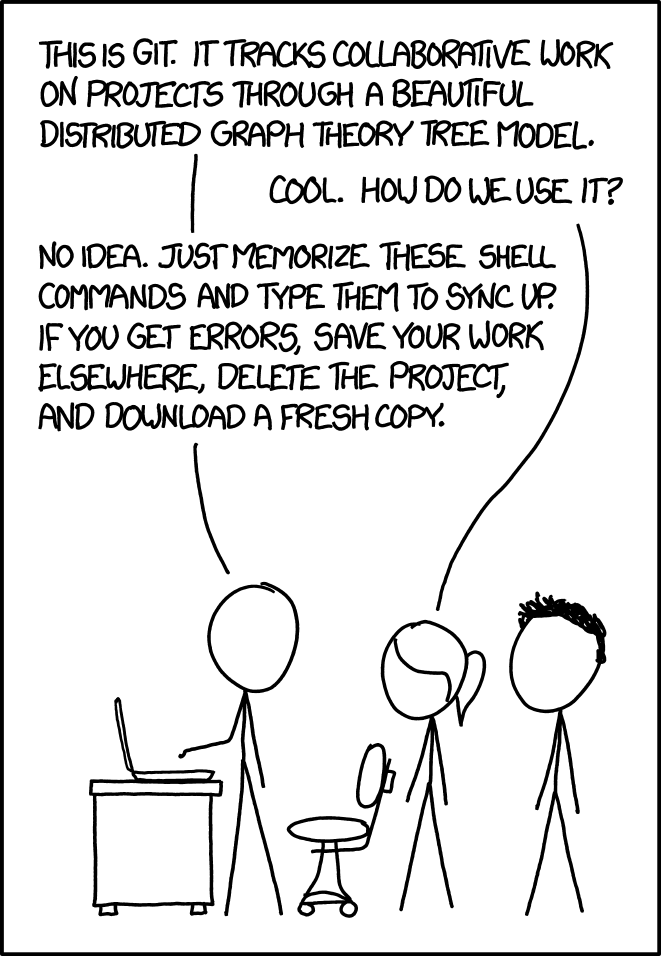
\includegraphics[width = 0.5 \linewidth]{images/git_2x.png}

\section{Formulas}

A Kuh is a Vieh vom Mü-Viertl, d.h.

\begin{align}
  aq = a \phi \left( \frac{\mu}{4} \right)
\end{align}

\end{document}
